`\section{Results}
We are currently finding low workload, high workload, middle workload, delayed termination, and fast termination paths through the system using JPF. Using min and max duration flags it is possible to locate delayed and fast termination paths. Delayed paths indicate an inefficient team, while fast paths indicate an efficient team. While fast and slow paths are important to understand, low, high, and middle workload areas are, for the sake of this research, more important. Areas of low workload indicate an overabundance of human resources to accomplish a specific task. High workload is indicative of too few resources being allocated for a given task. Both aspects need to be minimized in order to optimize the current system. 

There are two different simulations that gave us interesting results. The first is when the Video Operator was able to identify the target during a flight without any complications occurring (see Figure~\ref{fig:WorkloadSim1}) For the first 40 time steps everything behaves as expected. The peaks result from periods of communication between actors as they exchange the information necessary to start the search. At time step forty we see a fascinating deviation from the norm. At that point the temporal workload dominates the system. This is a result of constant information passing between the GUIs and the operators. Since there is a constant passing of data between the machinery and the operators, it is only logical that the workload would increase substantially. However the results indicate that a weighting should be instigated to balance the three workload measures rather than allowing the single category to dominate the system. In our sensitivity study we will verify whether this is a fault in our metrics or if this one scenario lends itself to the distortion.

\begin{figure}[h]
\center
\setlength{\abovecaptionskip}{1mm}
\setlength{\belowcaptionskip}{1mm}
\setlength{\textfloatsep}{1mm}
\setlength{\floatsep}{1mm}
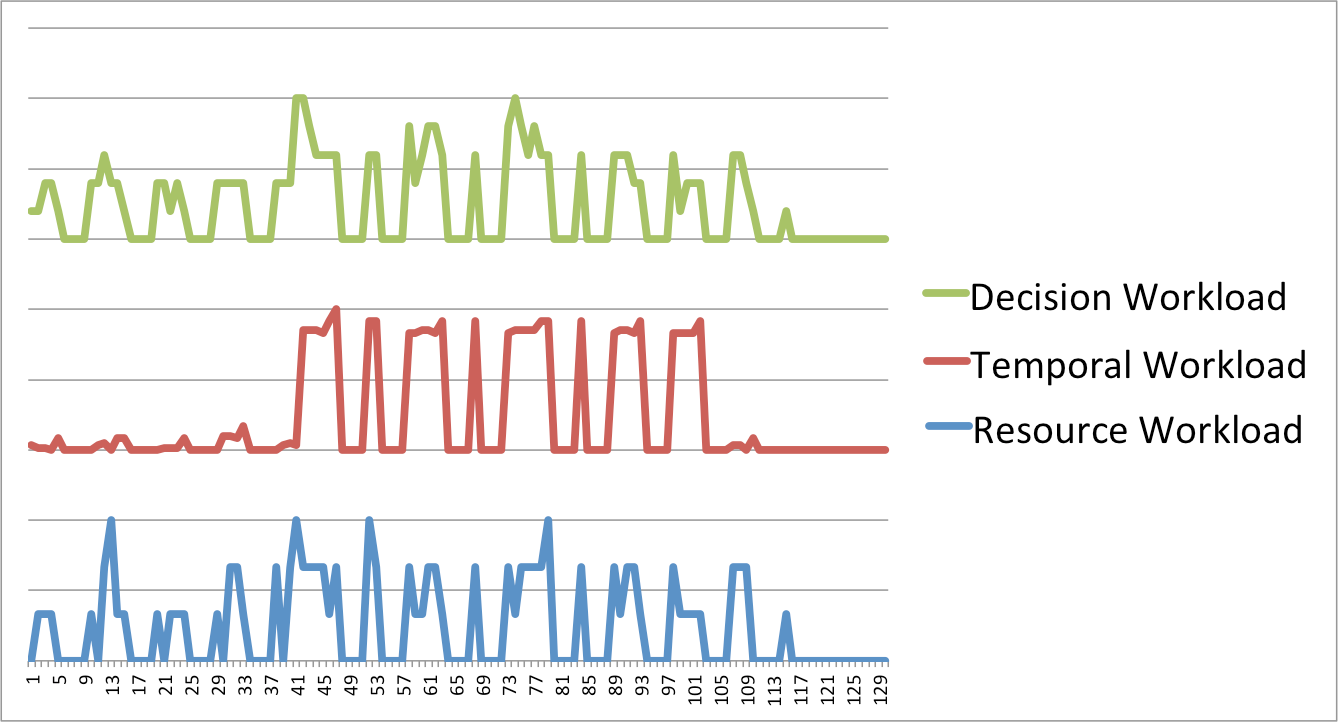
\includegraphics[height=2in]{WorkloadTargetSightingLabeled.png}
\caption{Workload over an uneventful flight}
\label{fig:WorkloadSim1}
\end{figure}

The second simulation we ran dealt with a situation where after a short period of flight time the battery rapidly fails. In this particular situation the operator was unable to respond quickly enough to land the UAV before it crashed(see Figure~\ref{fig:WorkloadSim2}). As with the previous simulation we saw an immediate spike in the temporal workload however in this simulation the workload decreased back to normal levels in just five time steps. The second spike that occurred indicated a sudden fluctuation in options among one of the actors which will have to be investigated further to verify if this is an accurate response or if a flaw in the model had slipped past the verification stage of development. Finally as would be expected when the UAV crashed there was a small spike in the workload before everything came to a halt. This last part of the simulation behaved precisely as expected.

\begin{figure}[h]
\center
\setlength{\abovecaptionskip}{1mm}
\setlength{\belowcaptionskip}{1mm}
\setlength{\textfloatsep}{1mm}
\setlength{\floatsep}{1mm}
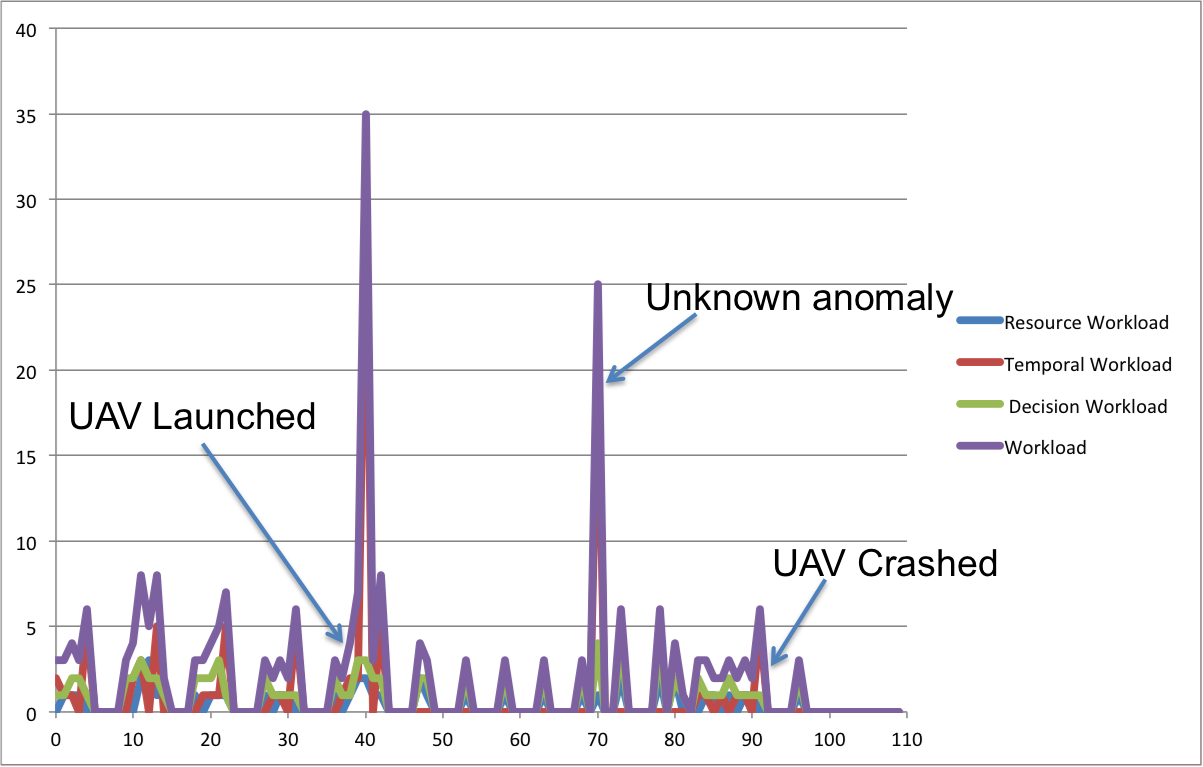
\includegraphics[height=2in]{WorkloadCrashedLabeled.png}
\caption{Emergency battery failure simulation}
\label{fig:WorkloadSim2}
\end{figure}